\section{Modeling}
\subsection{Voting Classifier}

I built a voting classifier using three different models: Random Forest, Logistic Regression, and Neural Network.

\paragraph{Random Forest}
I performed a Randomized Search with Stratified K-Fold cross-validation. Additionally, I tried an Extra Trees Classifier. Key observations include:
\begin{itemize}
    \item Random Forests easily overfit the training data.
    \item Regularization techniques very important here.
    \item Increasing the minimum number of samples per leaf helped prevent overfitting.
    \item Normal Random forest outperforms then Extra Trees Classifier.
\end{itemize}

\paragraph{Logistic Regression and KNN}
These classifiers initially achieved poor performance. Notable improvements came from:
\begin{itemize}
    \item Using RobustScaler, which helped more than other scaling techniques.
    \item Setting the \texttt{class\_weight} parameter, which was crucial for performance.
\end{itemize}

\paragraph{Multi-Layer Perceptrons (MLP) - Neural networks}
The MLP achieved the most balance between training and validation performance. Key points from the randomized search with Stratified K-Fold:
\begin{itemize}
    \item Stochastic Gradient Descent (SGD) optimizer performed better than Adam.
    \item The \texttt{tanh} activation function worked better than ReLU.
\end{itemize}


\subsection{Results}
\begin{figure}[h]
    \centering
    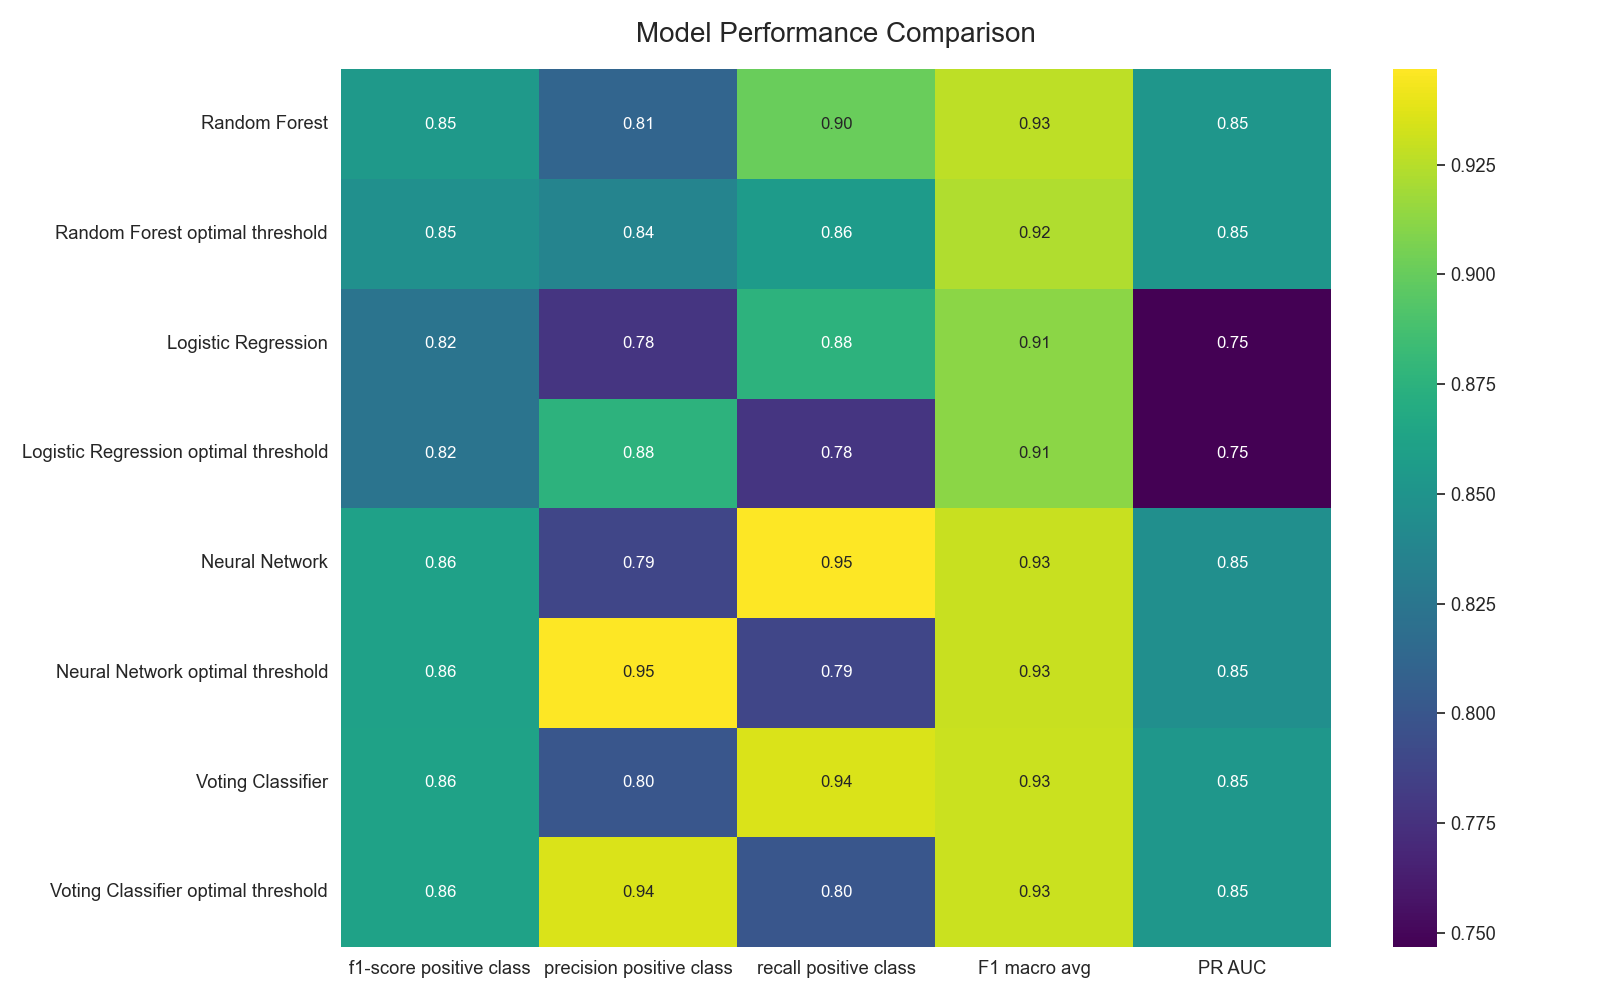
\includegraphics[width=0.74\linewidth]{approach one reaults.png}
    \caption{Model comparison on validation data}
    \label{fig: Model comparison on validation data}
\end{figure}


\newpage
\noindent\textbf{Note:}
\hfill \break
The optimal threshold is calculated by finding the highest F1-score and its threshold in training data only.

\begin{figure}[h]
    \centering
    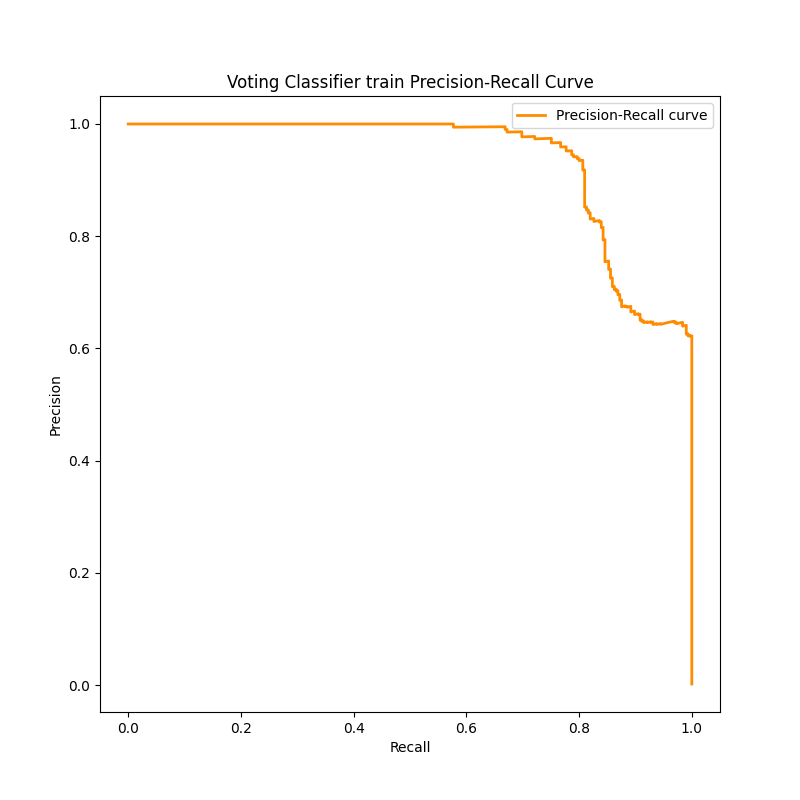
\includegraphics[width=0.5\linewidth]{Voting Classifier train precision recall area under curve.png}
    \caption{Voting Classifier PR-AUC}
    \label{fig:Voting Classifier PR-AUC}
\end{figure}

\begin{figure}[h]
    \centering
    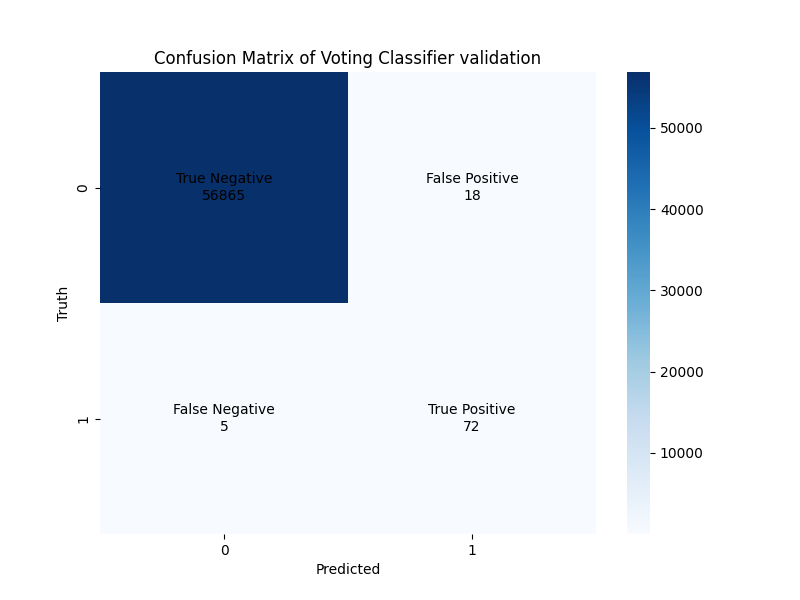
\includegraphics[width=0.65\linewidth]{Voting Classifier validation confusion matrix.png}
    \caption{Voting classifier validation confusion matrix}
    \label{fig:Voting classifier validation confusion matrix}
\end{figure}

\noindent\textbf{Observation:}
\hfill \break
I also observed using K-Nearest Neighbors (KNN) with the \texttt{ball\_tree} algorithm achieved a performance close to that of Random Forest and the neural network but required significantly high computational power.


\newpage
\subsection{Neural network with focal loss}
Focal Loss is a specialized loss function designed to address the class imbalance problem commonly encountered in tasks like object detection. It was introduced in the paper "Focal Loss for Dense Object Detection." The main idea is to focus more on hard-to-classify examples while reducing the loss contribution from easy-to-classify examples. This is achieved through two parameters $\alpha$ (alpha) and $\gamma$ (gamma).

\begin{figure}[h]
    \centering
    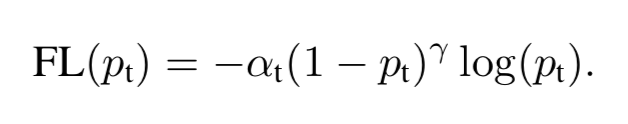
\includegraphics[width=1\linewidth]{Focal_Loss.png}
    \caption{Focal Loss formula}
    \label{fig:Focal Loss formula}
\end{figure}


\begin{lstlisting}[language=Python, caption=My Focal Loss Implementation in PyTorch]
class FocalLoss(nn.Module):
    def __init__(self, gamma=2, alpha=0.25):
        super(FocalLoss, self).__init__()
        self.gamma = gamma
        self.alpha = alpha

    def forward(self, pred_logits, target):
        BCELoss = F.binary_cross_entropy_with_logits(pred_logits, target, reduction='none')
        prob = pred_logits.sigmoid()
        alpha_t = torch.where(target == 1, self.alpha, (1 - self.alpha))
        pt =  torch.where(target == 1, prob, 1 - prob)
        loss = alpha_t * ((1 - pt) ** self.gamma) * BCELoss
        return loss.sum()
\end{lstlisting}

\noindent\textbf{Observation and Notes:}

\begin{itemize}
    \item I experimented with different combinations of $\alpha$ (0.80--0.99, increment of 0.05) and $\gamma$ (0--4, increment of 1).
    \item The best result was achieved with $\alpha = 0.75$ and $\gamma = 2$.
    \item $\alpha$ and $\gamma$ sometimes cause instability during training. Using Batch Normalization mitigated this effect, and switching from Adam to SGD also helped.
    \item A high $\gamma$ (5--7) results in a very noisy loss curve.
    \item A high $\alpha$ gives very high recall for positive class with less precision and vice versa.   
\end{itemize}

\begin{figure}[h]
    \centering
    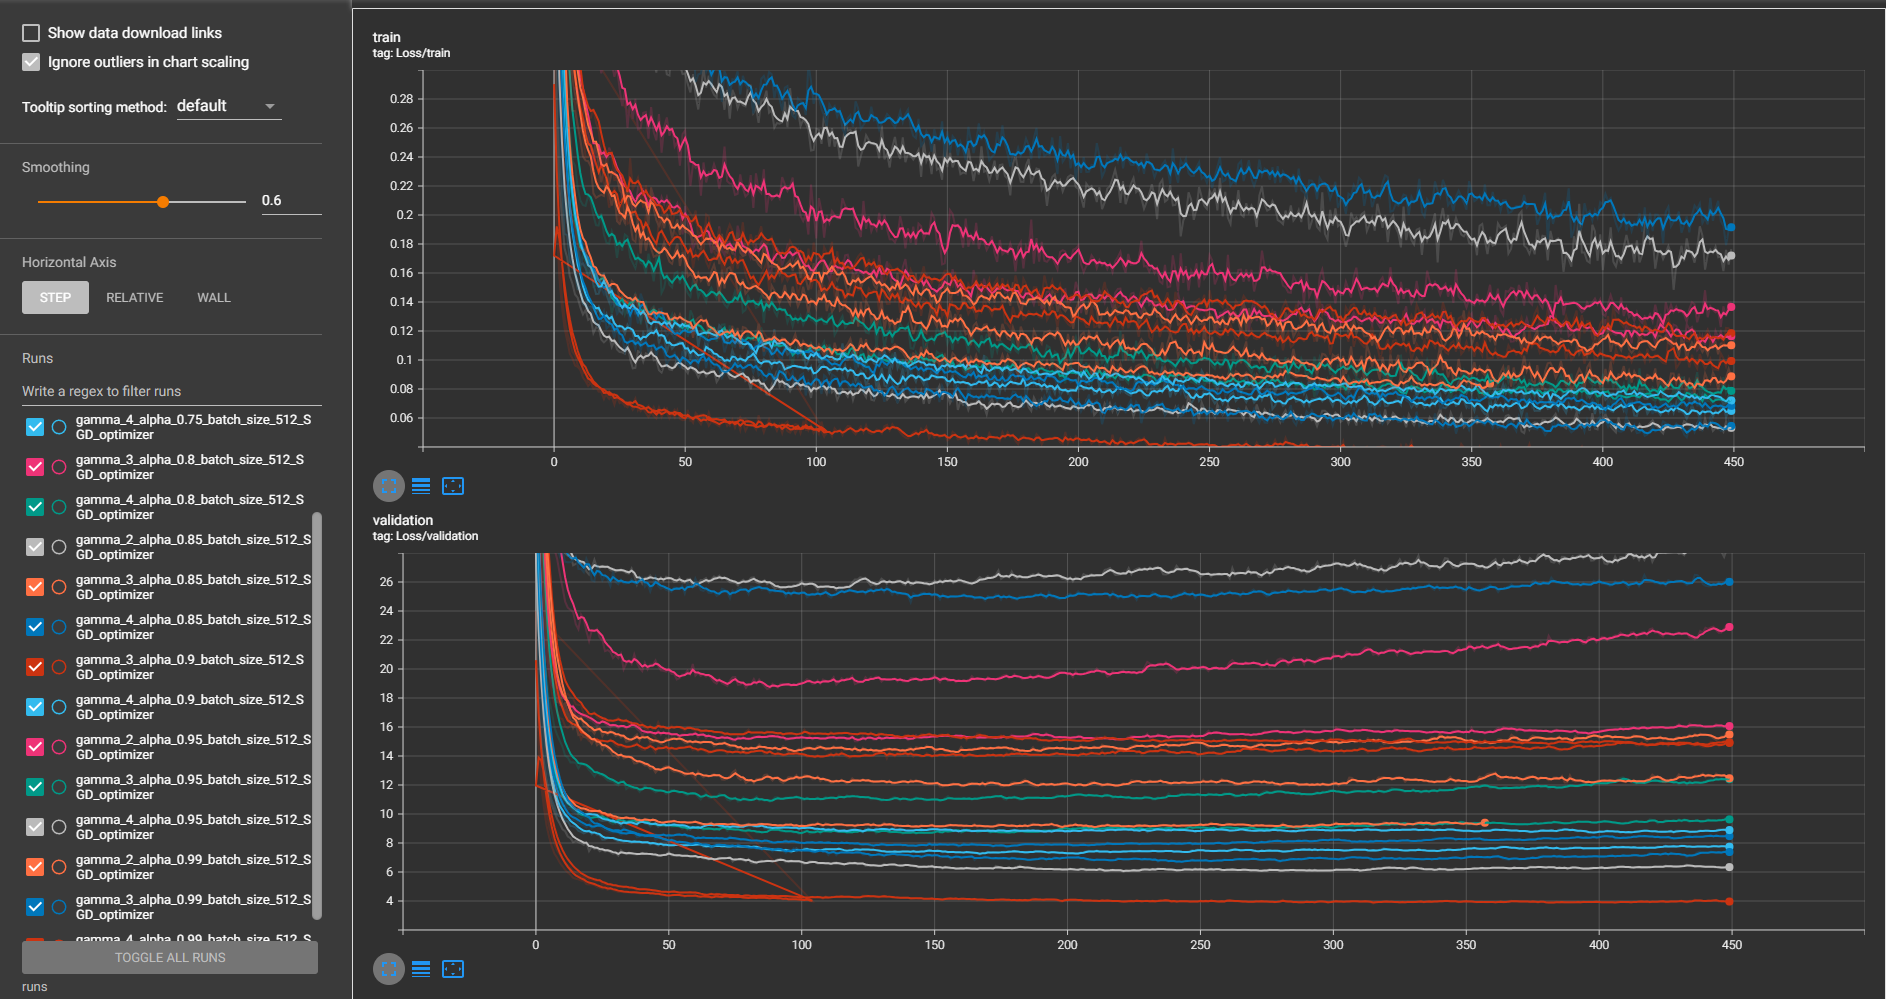
\includegraphics[width=1\linewidth]{different combination of Alpha and gamma.png}
    \caption{Different alpha and gamma effect Loss curve}
    \label{fig:Alpha and gamma}
\end{figure}

\subsection{Results}
\begin{figure}[h]
    \centering
    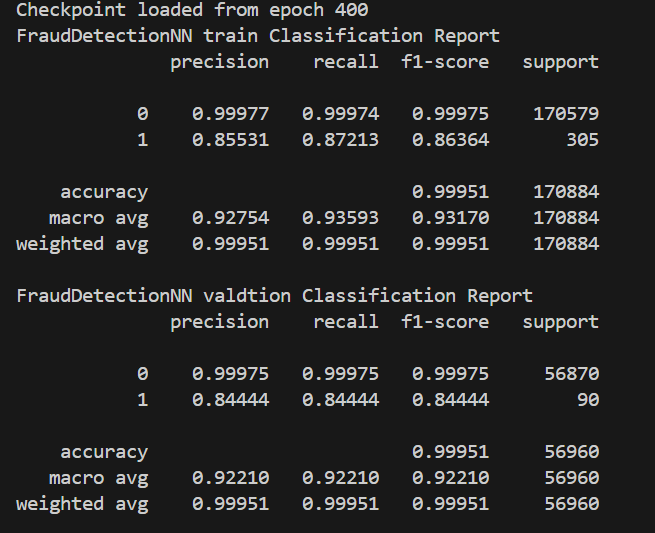
\includegraphics[width=0.8\linewidth]{Focal loss classification report.png}
    \caption{Focal loss classification report}
    \label{fig:Focal loss classification report}
\end{figure}


